%!TeX root=../sensetop.tex
\chapter[Chapter \thechapter]{}
\lettrine[lines=4,lraise=0.3]{E}{linor}, starting back with a look of horror at the sight of him, obeyed the first impulse of her heart in turning instantly to quit the room, and her hand was already on the lock, when its action was suspended by his hastily advancing, and saying, in a voice rather of command than supplication,

»Miss Dashwood, for half an hour—for ten minutes—I entreat you to stay.«

\begin{figure}[tbph]
\centering
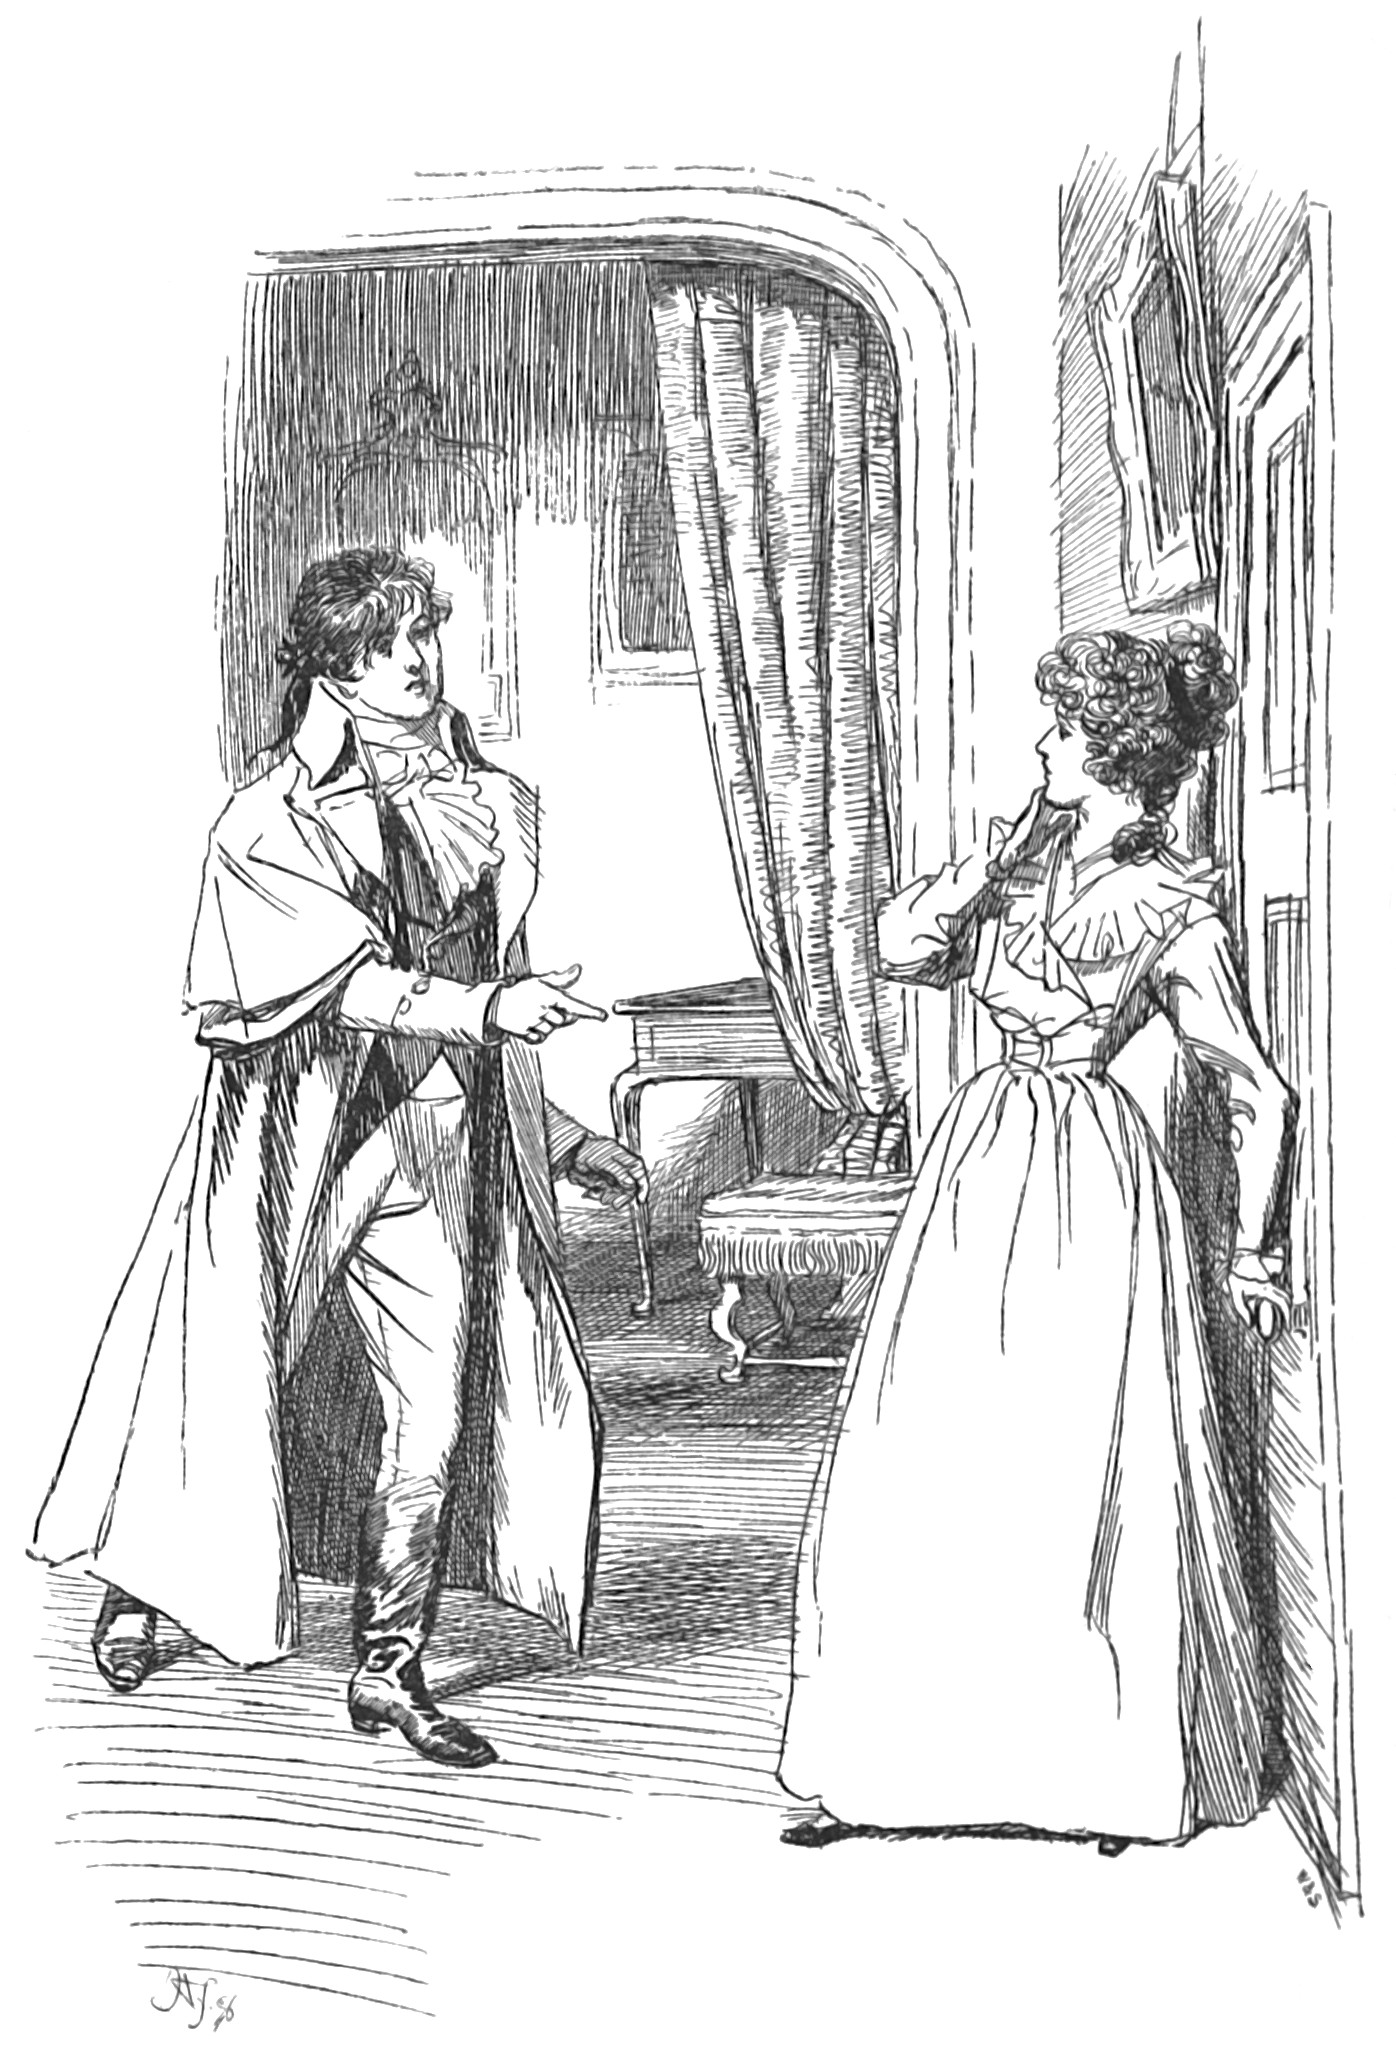
\includegraphics[width=\linewidth]{44stay}
\caption{»I entreat you to stay«}
\end{figure}

»No, sir,« she replied with firmness, »I shall \textit{not} stay. Your business cannot be with \textit{me}. The servants, I suppose, forgot to tell you that Mr Palmer was not in the house.«

»Had they told me,« he cried with vehemence, »that Mr Palmer and all his relations were at the devil, it would not have turned me from the door. My business is with you, and only you.«

»With me!«—in the utmost amazement—»well, sir,—be quick—and if you can—less violent.«

»Sit down, and I will be both.«

She hesitated; she knew not what to do. The possibility of Colonel Brandon’s arriving and finding her there, came across her. But she had promised to hear him, and her curiosity no less than her honour was engaged. After a moment’s recollection, therefore, concluding that prudence required dispatch, and that her acquiescence would best promote it, she walked silently towards the table, and sat down. He took the opposite chair, and for half a minute not a word was said by either.

»Pray be quick, sir,«—said Elinor, impatiently;—»I have no time to spare.«

He was sitting in an attitude of deep meditation, and seemed not to hear her.

»Your sister,« said he, with abruptness, a moment afterwards—»is out of danger. I heard it from the servant. God be praised!—But is it true? is it really true?«

Elinor would not speak. He repeated the inquiry with yet greater eagerness.

»For God’s sake tell me, is she out of danger, or is she not?«

»We hope she is.«

He rose up, and walked across the room.

»Had I known as much half an hour ago;—but since I \textit{am} here,« speaking with a forced vivacity as he returned to his seat,—»what does it signify? For once, Miss Dashwood—it will be the last time, perhaps—let us be cheerful together. I am in a fine mood for gaiety. Tell me honestly« a deeper glow overspreading his cheeks, »do you think me most a knave or a fool?«

Elinor looked at him with greater astonishment than ever. She began to think that he must be in liquor;—the strangeness of such a visit, and of such manners, seemed no otherwise intelligible; and with this impression she immediately rose, saying,

»Mr Willoughby, I advise you at present to return to Combe. I am not at leisure to remain with you longer. Whatever your business may be with me, it will be better recollected and explained to-morrow.«

»I understand you,« he replied, with an expressive smile, and a voice perfectly calm; »yes, I am very drunk. A pint of porter with my cold beef at Marlborough was enough to over-set me.«

»At Marlborough!«—cried Elinor, more and more at a loss to understand what he would be at.

»Yes,—I left London this morning at eight o’clock, and the only ten minutes I have spent out of my chaise since that time procured me a nuncheon at Marlborough.«

The steadiness of his manner, and the intelligence of his eye as he spoke, convincing Elinor, that whatever other unpardonable folly might bring him to Cleveland, he was not brought there by intoxication, she said, after a moment’s recollection,

»Mr Willoughby, you \textit{ought} to feel, and I certainly \textit{do}, that after what has passed, your coming here in this manner, and forcing yourself upon my notice, requires a very particular excuse. What is it, that you mean by it?«

»I mean,« said he, with serious energy, »if I can, to make you hate me one degree less than you do \textit{now}. I mean to offer some kind of explanation, some kind of apology, for the past; to open my whole heart to you, and by convincing you, that though I have been always a blockhead, I have not been always a rascal, to obtain something like forgiveness from Ma— from your sister.«

»Is this the real reason of your coming?«

»Upon my soul it is,«—was his answer, with a warmth which brought all the former Willoughby to her remembrance, and in spite of herself made her think him sincere.

»If that is all, you may be satisfied already; for Marianne \textit{does}, she has \textit{long} forgiven you.«

»Has she?« he cried, in the same eager tone. »Then she has forgiven me before she ought to have done it. But she shall forgive me again, and on more reasonable grounds. \textit{Now} will you listen to me?«

Elinor bowed her assent.

»I do not know,« said he, after a pause of expectation on her side, and thoughtfulness on his own, »how \textit{you} may have accounted for my behaviour to your sister, or what diabolical motive you may have imputed to me. Perhaps you will hardly think the better of me,—it is worth the trial however, and you shall hear every thing. When I first became intimate in your family, I had no other intention, no other view in the acquaintance than to pass my time pleasantly while I was obliged to remain in Devonshire, more pleasantly than I had ever done before. Your sister’s lovely person and interesting manners could not but please me; and her behaviour to me almost from the first, was of a kind—it is astonishing, when I reflect on what it was, and what \textit{she} was, that my heart should have been so insensible! But at first I must confess, my vanity only was elevated by it. Careless of her happiness, thinking only of my own amusement, giving way to feelings which I had always been too much in the habit of indulging, I endeavoured, by every means in my power, to make myself pleasing to her, without any design of returning her affection.«

Miss Dashwood, at this point, turning her eyes on him with the most angry contempt, stopped him, by saying,

»It is hardly worth while, Mr Willoughby, for you to relate, or for me to listen any longer. Such a beginning as this cannot be followed by any thing. Do not let me be pained by hearing any thing more on the subject.«

»I insist on you hearing the whole of it,« he replied, »My fortune was never large, and I had always been expensive, always in the habit of associating with people of better income than myself. Every year since my coming of age, or even before, I believe, had added to my debts; and though the death of my old cousin, Mrs Smith, was to set me free; yet that event being uncertain, and possibly far distant, it had been for some time my intention to re-establish my circumstances by marrying a woman of fortune. To attach myself to your sister, therefore, was not a thing to be thought of; and with a meanness, selfishness, cruelty, which no indignant, no contemptuous look, even of yours, Miss Dashwood, can ever reprobate too much,—I was acting in this manner, trying to engage her regard, without a thought of returning it. But one thing may be said for me: even in that horrid state of selfish vanity, I did not know the extent of the injury I meditated, because I did not \textit{then} know what it was to love. But have I ever known it? Well may it be doubted; for, had I really loved, could I have sacrificed my feelings to vanity, to avarice? or, what is more, could I have sacrificed hers? But I have done it. To avoid a comparative poverty, which her affection and her society would have deprived of all its horrors, I have, by raising myself to affluence, lost every thing that could make it a blessing.«

»You did then,« said Elinor, a little softened, »believe yourself at one time attached to her?«

»To have resisted such attractions, to have withstood such tenderness! Is there a man on earth who could have done it? Yes, I found myself, by insensible degrees, sincerely fond of her; and the happiest hours of my life were what I spent with her when I felt my intentions were strictly honourable, and my feelings blameless. Even \textit{then}, however, when fully determined on paying my addresses to her, I allowed myself most improperly to put off, from day to day, the moment of doing it, from an unwillingness to enter into an engagement while my circumstances were so greatly embarrassed. I will not reason here—nor will I stop for \textit{you} to expatiate on the absurdity, and the worse than absurdity, of scrupling to engage my faith where my honour was already bound. The event has proved, that I was a cunning fool, providing with great circumspection for a possible opportunity of making myself contemptible and wretched for ever. At last, however, my resolution was taken, and I had determined, as soon as I could engage her alone, to justify the attentions I had so invariably paid her, and openly assure her of an affection which I had already taken such pains to display. But in the interim—in the interim of the very few hours that were to pass, before I could have an opportunity of speaking with her in private—a circumstance occurred—an unlucky circumstance, to ruin all my resolution, and with it all my comfort. A discovery took place,«—here he hesitated and looked down. »Mrs Smith had somehow or other been informed, I imagine by some distant relation, whose interest it was to deprive me of her favour, of an affair, a connection—but I need not explain myself farther,« he added, looking at her with an heightened colour and an enquiring eye,—»your particular intimacy—you have probably heard the whole story long ago.«

»I have,« returned Elinor, colouring likewise, and hardening her heart anew against any compassion for him, »I have heard it all. And how you will explain away any part of your guilt in that dreadful business, I confess is beyond my comprehension.«

»Remember,« cried Willoughby, »from whom you received the account. Could it be an impartial one? I acknowledge that her situation and her character ought to have been respected by me. I do not mean to justify myself, but at the same time cannot leave you to suppose that I have nothing to urge—that because she was injured she was irreproachable, and because \textit{I} was a libertine, \textit{she} must be a saint. If the violence of her passions, the weakness of her understanding—I do not mean, however, to defend myself. Her affection for me deserved better treatment, and I often, with great self-reproach, recall the tenderness which, for a very short time, had the power of creating any return. I wish—I heartily wish it had never been. But I have injured more than herself; and I have injured one, whose affection for me (may I say it?) was scarcely less warm than hers; and whose mind—Oh! how infinitely superior!«

»Your indifference, however, towards that unfortunate girl—I must say it, unpleasant to me as the discussion of such a subject may well be—your indifference is no apology for your cruel neglect of her. Do not think yourself excused by any weakness, any natural defect of understanding on her side, in the wanton cruelty so evident on yours. You must have known, that while you were enjoying yourself in Devonshire pursuing fresh schemes, always gay, always happy, she was reduced to the extremest indigence.«

»But, upon my soul, I did \textit{not} know it,« he warmly replied; »I did not recollect that I had omitted to give her my direction; and common sense might have told her how to find it out.«

»Well, sir, and what said Mrs Smith?«

»She taxed me with the offence at once, and my confusion may be guessed. The purity of her life, the formality of her notions, her ignorance of the world—every thing was against me. The matter itself I could not deny, and vain was every endeavour to soften it. She was previously disposed, I believe, to doubt the morality of my conduct in general, and was moreover discontented with the very little attention, the very little portion of my time that I had bestowed on her, in my present visit. In short, it ended in a total breach. By one measure I might have saved myself. In the height of her morality, good woman! she offered to forgive the past, if I would marry Eliza. That could not be—and I was formally dismissed from her favour and her house. The night following this affair—I was to go the next morning—was spent by me in deliberating on what my future conduct should be. The struggle was great—but it ended too soon. My affection for Marianne, my thorough conviction of her attachment to me—it was all insufficient to outweigh that dread of poverty, or get the better of those false ideas of the necessity of riches, which I was naturally inclined to feel, and expensive society had increased. I had reason to believe myself secure of my present wife, if I chose to address her, and I persuaded myself to think that nothing else in common prudence remained for me to do. A heavy scene however awaited me, before I could leave Devonshire;—I was engaged to dine with you on that very day; some apology was therefore necessary for my breaking this engagement. But whether I should write this apology, or deliver it in person, was a point of long debate. To see Marianne, I felt, would be dreadful, and I even doubted whether I could see her again, and keep to my resolution. In that point, however, I undervalued my own magnanimity, as the event declared; for I went, I saw her, and saw her miserable, and left her miserable—and left her hoping never to see her again.«

\begin{figure}[tbph]
\centering
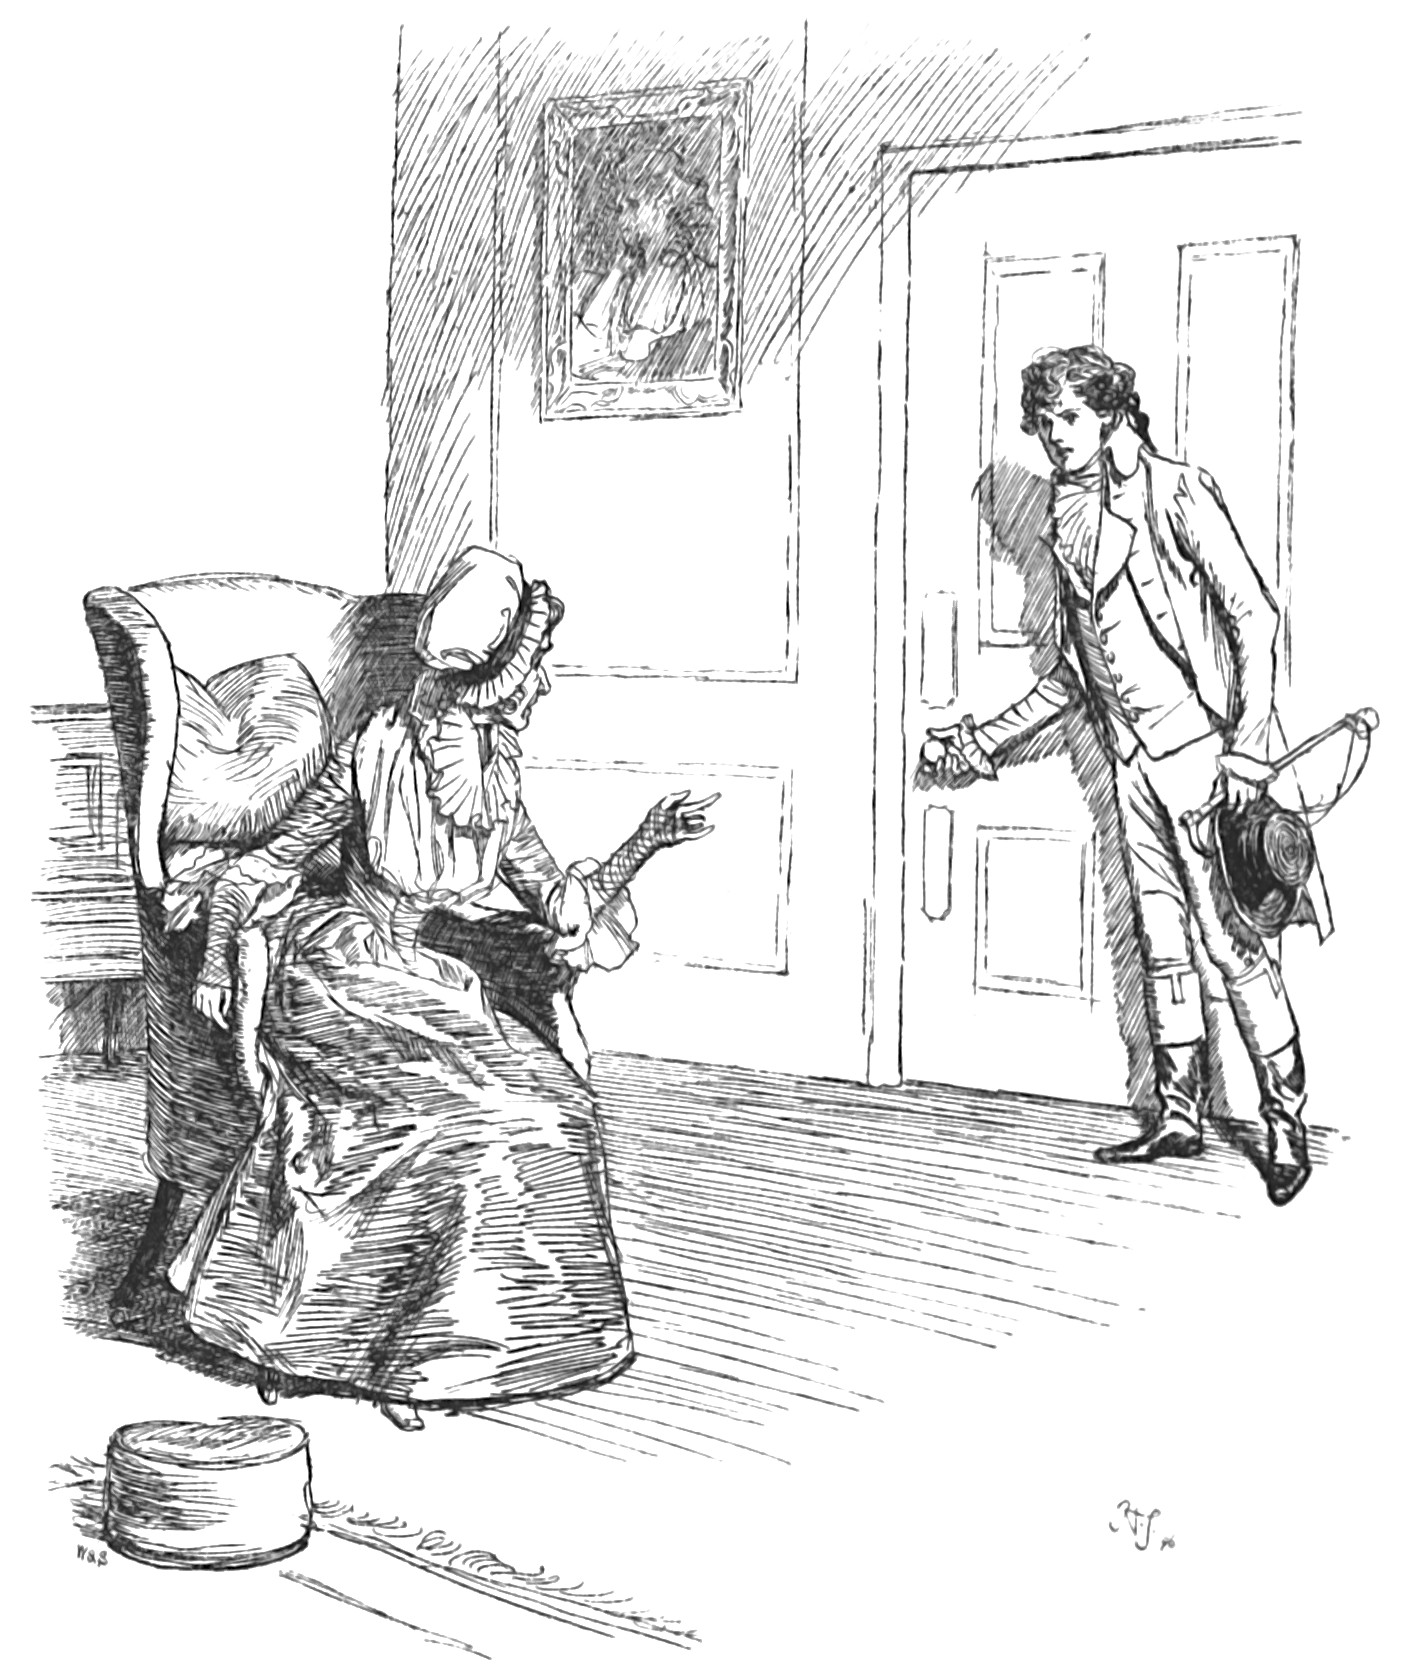
\includegraphics[width=\linewidth]{44dismissed}
\caption{»I was formally dismissed«}
\end{figure}

»Why did you call, Mr Willoughby?« said Elinor, reproachfully; »a note would have answered every purpose. Why was it necessary to call?«

»It was necessary to my own pride. I could not bear to leave the country in a manner that might lead you, or the rest of the neighbourhood, to suspect any part of what had really passed between Mrs Smith and myself—and I resolved therefore on calling at the cottage, in my way to Honiton. The sight of your dear sister, however, was really dreadful; and, to heighten the matter, I found her alone. You were all gone I do not know where. I had left her only the evening before, so fully, so firmly resolved within my self on doing right! A few hours were to have engaged her to me for ever; and I remember how happy, how gay were my spirits, as I walked from the cottage to Allenham, satisfied with myself, delighted with every body! But in this, our last interview of friendship, I approached her with a sense of guilt that almost took from me the power of dissembling. Her sorrow, her disappointment, her deep regret, when I told her that I was obliged to leave Devonshire so immediately—I never shall forget it—united too with such reliance, such confidence in me!—Oh, God!—what a hard-hearted rascal I was!«

They were both silent for a few moments. Elinor first spoke.

»Did you tell her that you should soon return?«

»I do not know what I told her,« he replied, impatiently; »less than was due to the past, beyond a doubt, and in all likelihood much more than was justified by the future. I cannot think of it.—It won’t do.—Then came your dear mother to torture me farther, with all her kindness and confidence. Thank Heaven! it \textit{did} torture me. I was miserable. Miss Dashwood, you cannot have an idea of the comfort it gives me to look back on my own misery. I owe such a grudge to myself for the stupid, rascally folly of my own heart, that all my past sufferings under it are only triumph and exultation to me now. Well, I went, left all that I loved, and went to those to whom, at best, I was only indifferent. My journey to town—travelling with my own horses, and therefore so tediously—no creature to speak to—my own reflections so cheerful—when I looked forward every thing so inviting!—when I looked back at Barton, the picture so soothing!—oh, it was a blessed journey!«

He stopped.

»Well, sir,« said Elinor, who, though pitying him, grew impatient for his departure, »and this is all?«

»All!—no:—have you forgot what passed in town? That infamous letter? Did she show it you?«

»Yes, I saw every note that passed.«

»When the first of hers reached me (as it immediately did, for I was in town the whole time,) what I felt is—in the common phrase, not to be expressed; in a more simple one—perhaps too simple to raise any emotion—my feelings were very, very painful.—Every line, every word was—in the hackneyed metaphor which their dear writer, were she here, would forbid—a dagger to my heart. To know that Marianne was in town was—in the same language—a thunderbolt.—Thunderbolts and daggers!—what a reproof would she have given me!—her taste, her opinions—I believe they are better known to me than my own,—and I am sure they are dearer.«

Elinor’s heart, which had undergone many changes in the course of this extraordinary conversation, was now softened again;—yet she felt it her duty to check such ideas in her companion as the last.

»This is not right, Mr Willoughby.—Remember that you are married. Relate only what in your conscience you think necessary for me to hear.«

»Marianne’s note, by assuring me that I was still as dear to her as in former days,—that in spite of the many, many weeks we had been separated, she was as constant in her own feelings, and as full of faith in the constancy of mine as ever,—awakened all my remorse. I say awakened, because time and London, business and dissipation, had in some measure quieted it, and I had been growing a fine hardened villain, fancying myself indifferent to her, and chusing to fancy that she too must have become indifferent to me; talking to myself of our past attachment as a mere idle, trifling business, shrugging up my shoulders in proof of its being so, and silencing every reproach, overcoming every scruple, by secretly saying now and then, »I shall be heartily glad to hear she is well married.« But this note made me know myself better. I felt that she was infinitely dearer to me than any other woman in the world, and that I was using her infamously. But every thing was then just settled between Miss Grey and me. To retreat was impossible. All that I had to do, was to avoid you both. I sent no answer to Marianne, intending by that to preserve myself from her farther notice; and for some time I was even determined not to call in Berkeley Street;—but at last, judging it wiser to affect the air of a cool, common acquaintance than anything else, I watched you all safely out of the house one morning, and left my name.«

»Watched us out of the house!«

»Even so. You would be surprised to hear how often I watched you, how often I was on the point of falling in with you. I have entered many a shop to avoid your sight, as the carriage drove by. Lodging as I did in Bond Street, there was hardly a day in which I did not catch a glimpse of one or other of you; and nothing but the most constant watchfulness on my side, a most invariably prevailing desire to keep out of your sight, could have separated us so long. I avoided the Middletons as much as possible, as well as everybody else who was likely to prove an acquaintance in common. Not aware of their being in town, however, I blundered on Sir John, I believe, the first day of his coming, and the day after I had called at Mrs Jennings’s. He asked me to a party, a dance at his house in the evening. Had he \textit{not} told me as an inducement that you and your sister were to be there, I should have felt it too certain a thing, to trust myself near him. The next morning brought another short note from Marianne—still affectionate, open, artless, confiding—everything that could make \textit{my} conduct most hateful. I could not answer it. I tried—but could not frame a sentence. But I thought of her, I believe, every moment of the day. If you \textit{can} pity me, Miss Dashwood, pity my situation as it was \textit{then}. With my head and heart full of your sister, I was forced to play the happy lover to another woman! Those three or four weeks were worse than all. Well, at last, as I need not tell you, you were forced on me; and what a sweet figure I cut! what an evening of agony it was! Marianne, beautiful as an angel on one side, calling me Willoughby in such a tone! Oh, God! holding out her hand to me, asking me for an explanation, with those bewitching eyes fixed in such speaking solicitude on my face! and Sophia, jealous as the devil on the other hand, looking all that was—Well, it does not signify; it is over now. Such an evening! I ran away from you all as soon as I could; but not before I had seen Marianne’s sweet face as white as death. \textit{That} was the last, last look I ever had of her; the last manner in which she appeared to me. It was a horrid sight! yet when I thought of her to-day as really dying, it was a kind of comfort to me to imagine that I knew exactly how she would appear to those, who saw her last in this world. She was before me, constantly before me, as I travelled, in the same look and hue.«

\begin{a4}
	\begin{figure}[tbph]
		\centering
		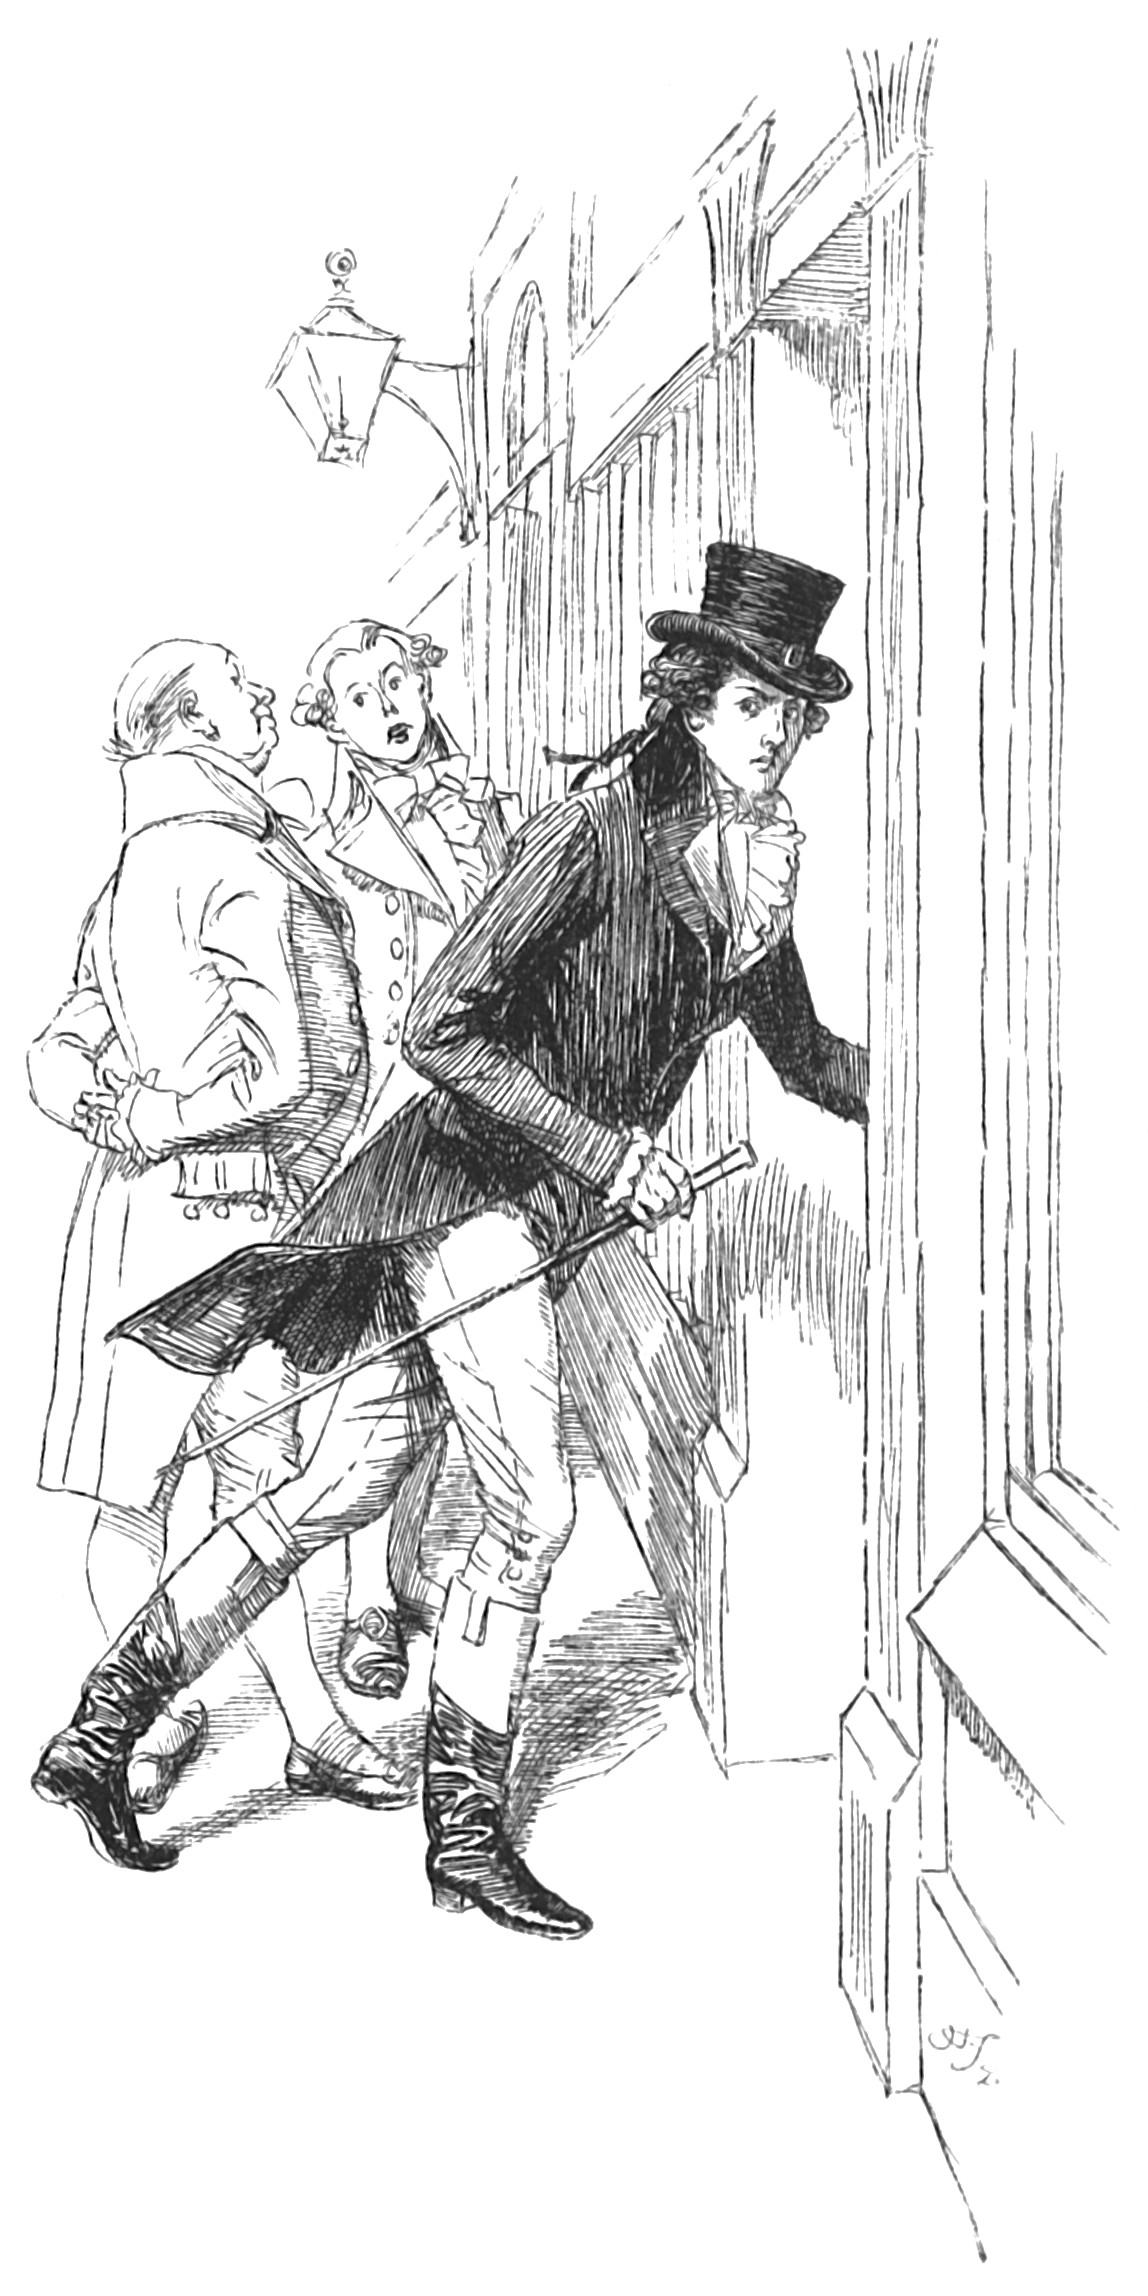
\includegraphics[width=.7\linewidth]{44shop}
		\caption{»I have entered many a shop to avoid your sight«}
	\end{figure}
\end{a4}

\begin{letter}
	\begin{figure}[tbph]
		\centering
		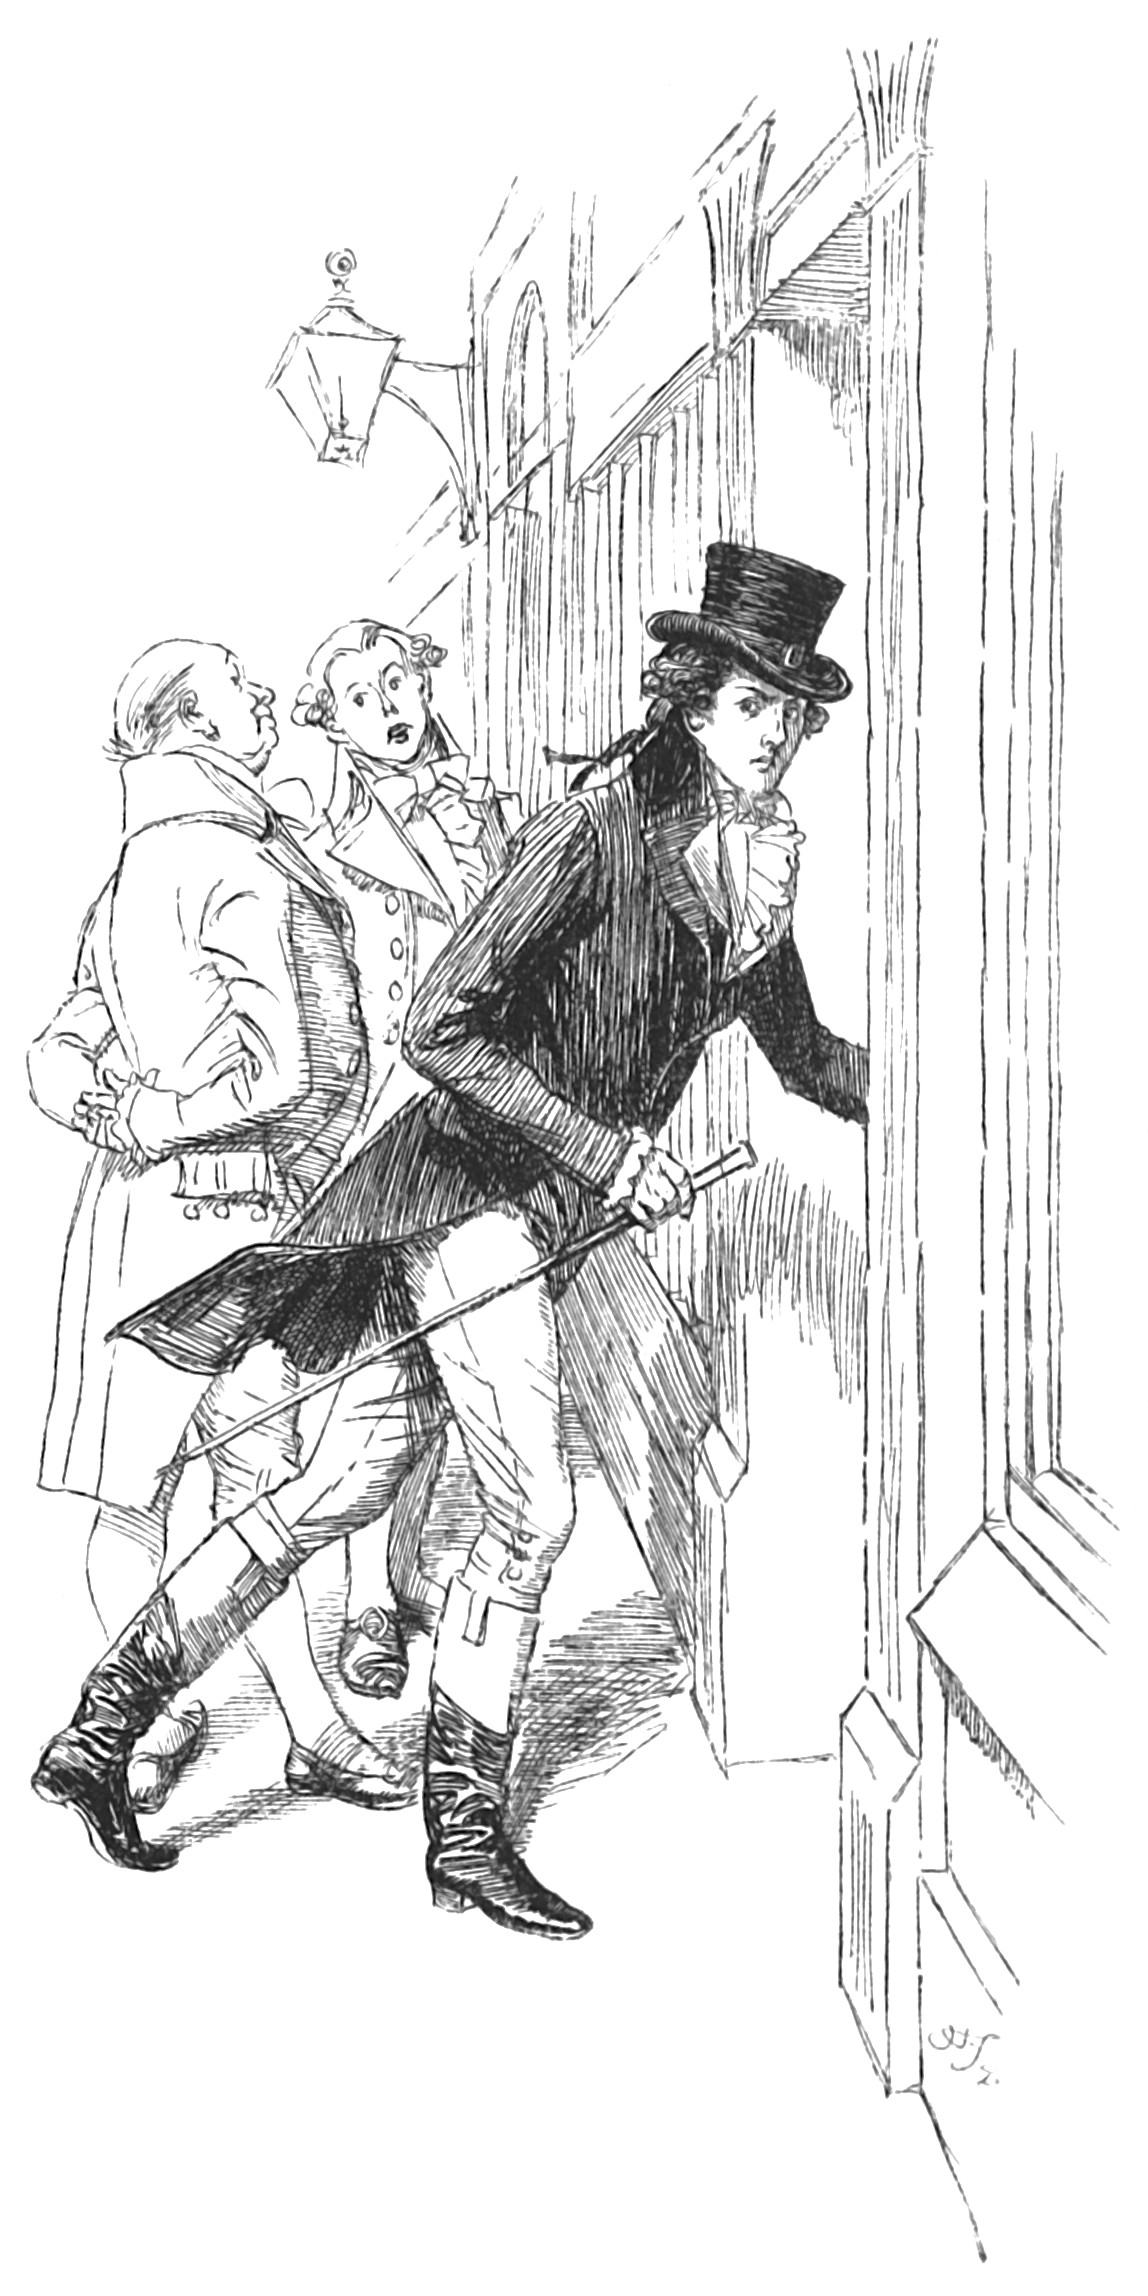
\includegraphics[width=.8\linewidth]{44shop}
		\caption{»I have entered many a shop to avoid your sight«}
	\end{figure}
\end{letter}

A short pause of mutual thoughtfulness succeeded. Willoughby first rousing himself, broke it thus:

»Well, let me make haste and be gone. Your sister is certainly better, certainly out of danger?«

»We are assured of it.«

»Your poor mother, too!—doting on Marianne.«

»But the letter, Mr Willoughby, your own letter; have you any thing to say about that?«

»Yes, yes, \textit{that} in particular. Your sister wrote to me again, you know, the very next morning. You saw what she said. I was breakfasting at the Ellisons,—and her letter, with some others, was brought to me there from my lodgings. It happened to catch Sophia’s eye before it caught mine—and its size, the elegance of the paper, the hand-writing altogether, immediately gave her a suspicion. Some vague report had reached her before of my attachment to some young lady in Devonshire, and what had passed within her observation the preceding evening had marked who the young lady was, and made her more jealous than ever. Affecting that air of playfulness, therefore, which is delightful in a woman one loves, she opened the letter directly, and read its contents. She was well paid for her impudence. She read what made her wretched. Her wretchedness I could have borne, but her passion—her malice—At all events it must be appeased. And, in short—what do you think of my wife’s style of letter-writing?—delicate—tender—truly feminine—was it not?«

»Your wife!—The letter was in your own hand-writing.«

»Yes, but I had only the credit of servilely copying such sentences as I was ashamed to put my name to. The original was all her own—her own happy thoughts and gentle diction. But what could I do!—we were engaged, every thing in preparation, the day almost fixed—But I am talking like a fool. Preparation! Day! In honest words, her money was necessary to me, and in a situation like mine, any thing was to be done to prevent a rupture. And after all, what did it signify to my character in the opinion of Marianne and her friends, in what language my answer was couched? It must have been only to one end. My business was to declare myself a scoundrel, and whether I did it with a bow or a bluster was of little importance. »I am ruined for ever in their opinion,« said I to myself: »I am shut out for ever from their society, they already think me an unprincipled fellow, this letter will only make them think me a blackguard one.« Such were my reasonings, as, in a sort of desperate carelessness, I copied my wife’s words, and parted with the last relics of Marianne. Her three notes,—unluckily they were all in my pocketbook, or I should have denied their existence, and hoarded them for ever,—I was forced to put them up, and could not even kiss them. And the lock of hair—that too I had always carried about me in the same pocket-book, which was now searched by Madam with the most ingratiating virulence,—the dear lock,—all, every memento was torn from me.«

»You are very wrong, Mr Willoughby, very blamable,« said Elinor, while her voice, in spite of herself, betrayed her compassionate emotion; »you ought not to speak in this way, either of Mrs Willoughby or my sister. You had made your own choice. It was not forced on you. Your wife has a claim to your politeness, to your respect, at least. She must be attached to you, or she would not have married you. To treat her with unkindness, to speak of her slightingly is no atonement to Marianne—nor can I suppose it a relief to your own conscience.«

»Do not talk to me of my wife,« said he with a heavy sigh; »she does not deserve your compassion. She knew I had no regard for her when we married. Well, married we were, and came down to Combe Magna to be happy, and afterwards returned to town to be gay. And now do you pity me, Miss Dashwood? Or have I said all this to no purpose? Am I,—be it only one degree,—am I less guilty in your opinion than I was before? My intentions were not always wrong. Have I explained away any part of my guilt?«

»Yes, you have certainly removed something—a little. You have proved yourself, on the whole, less faulty than I had believed you. You have proved your heart less wicked, much less wicked. But I hardly know—the misery that you have inflicted—I hardly know what could have made it worse.«

»Will you repeat to your sister when she is recovered, what I have been telling you?—Let me be a little lightened too in her opinion as well as in yours. You tell me that she has forgiven me already. Let me be able to fancy that a better knowledge of my heart, and of my present feelings, will draw from her a more spontaneous, more natural, more gentle, less dignified, forgiveness. Tell her of my misery and my penitence—tell her that my heart was never inconstant to her, and if you will, that at this moment she is dearer to me than ever.«

»I will tell her all that is necessary to what may comparatively be called, your justification. But you have not explained to me the particular reason of your coming now, nor how you heard of her illness.«

»Last night, in Drury Lane lobby, I ran against Sir John Middleton, and when he saw who I was, for the first time these two months, he spoke to me. That he had cut me ever since my marriage, I had seen without surprise or resentment. Now, however, his good-natured, honest, stupid soul, full of indignation against me, and concern for your sister, could not resist the temptation of telling me what he knew ought to, though probably he did not think it \textit{would}, vex me horridly. As bluntly as he could speak it, therefore, he told me that Marianne Dashwood was dying of a putrid fever at Cleveland—a letter that morning received from Mrs Jennings declared her danger most imminent—the Palmers are all gone off in a fright, \&c. I was too much shocked to be able to pass myself off as insensible even to the undiscerning Sir John. His heart was softened in seeing mine suffer; and so much of his ill-will was done away, that when we parted, he almost shook me by the hand while he reminded me of an old promise about a pointer puppy. What I felt on hearing that your sister was dying, and dying too, believing me the greatest villain upon earth, scorning, hating me in her latest moments—for how could I tell what horrid projects might not have been imputed? \textit{One} person I was sure would represent me as capable of anything—What I felt was dreadful! My resolution was soon made, and at eight o’clock this morning I was in my carriage. Now you know all.«

Elinor made no answer. Her thoughts were silently fixed on the irreparable injury which too early an independence and its consequent habits of idleness, dissipation, and luxury, had made in the mind, the character, the happiness, of a man who, to every advantage of person and talents, united a disposition naturally open and honest, and a feeling, affectionate temper. The world had made him extravagant and vain—Extravagance and vanity had made him cold-hearted and selfish. Vanity, while seeking its own guilty triumph at the expense of another, had involved him in a real attachment, which extravagance, or at least its offspring, necessity, had required to be sacrificed. Each faulty propensity in leading him to evil, had led him likewise to punishment. The attachment, from which against honour, against feeling, against every better interest he had outwardly torn himself, now, when no longer allowable, governed every thought; and the connection, for the sake of which he had, with little scruple, left her sister to misery, was likely to prove a source of unhappiness to himself of a far more incurable nature. From a reverie of this kind she was recalled at the end of some minutes by Willoughby, who, rousing himself from a reverie at least equally painful, started up in preparation for going, and said—

»There is no use in staying here; I must be off.«

»Are you going back to town?«

»No—to Combe Magna. I have business there; from thence to town in a day or two. Good bye.«

He held out his hand. She could not refuse to give him hers;—he pressed it with affection.

»And you \textit{do} think something better of me than you did?« said he, letting it fall, and leaning against the mantel-piece as if forgetting he was to go.

Elinor assured him that she did;—that she forgave, pitied, wished him well—was even interested in his happiness—and added some gentle counsel as to the behaviour most likely to promote it. His answer was not very encouraging.

»As to that,« said he, »I must rub through the world as well as I can. Domestic happiness is out of the question. If, however, I am allowed to think that you and yours feel an interest in my fate and actions, it may be the means—it may put me on my guard—at least, it may be something to live for. Marianne to be sure is lost to me for ever. Were I even by any blessed chance at liberty again\longdash«

Elinor stopped him with a reproof.

»Well,«—he replied—»once more good bye. I shall now go away and live in dread of one event.«

»What do you mean?«

»Your sister’s marriage.«

»You are very wrong. She can never be more lost to you than she is now.«

»But she will be gained by some one else. And if that some one should be the very he whom, of all others, I could least bear—but I will not stay to rob myself of all your compassionate goodwill, by showing that where I have most injured I can least forgive. Good bye,—God bless you!«

And with these words, he almost ran out of the room.